In this section the operational items are sized. This can be summarised as the mass needed by the astronauts to stay alive in the crew module during the mission. For this purpose the paper by Tito et al \cite{Tito2013} has been used. In this paper the operational items are called \gls{eclss}. First the method for estimation is described with its assumptions. Followed by the results of the estimation.

\paragraph{Estimation method}
\label{par:operationalest}
The mass of the \gls{eclss} is primarily driven by the crew size and mission length. The \gls{eclss} is divided into subsystems: Air Management, Thermal and Humidity Management, Water Management, Waste Management, Human Accommodation, Food Preparation and Storage. Each of these subsystems can be subdivided into components. Examples of these are a water heater or packed food in the Food Preparation and Storage. It is evident that some components scale with the key drivers and others do not. For example, adding a crew member does not necessitate an extra water heater, but it does require extra packed food. Taking this into account the mass has been divided into two components: A basic system mass which scales with crew size and the consumable mass that scales with crew size and mission length.

\paragraph{Results}
By using the methods from section \ref{par:operationalest} the results of table \ref{tab:operationalest} were obtained.
The masses associated with operational items can be split up into two sections: Basic system mass and consumables mass. Basic system mass consists of the systems concerning crew well-being and life support, such as: Oxygen scrubbers (not including oxygen), atmospheric control systems and food preparation systems. Consumables mass is concerned with items such as oxygen, food, water and personal provisions.
\begin{table}[h]
	\centering
	\caption{Obtained masses and volumes of basic system \& consumable items}
	\begin{tabular}{|p{2cm}|p{2cm}|p{2cm}|p{2.5cm}|p{2.5cm}|}
		\hline
		\textbf{Crew members} & \textbf{Basic system mass $[kg]$} & \textbf{Basic system volume $[m^{3}]$} & \textbf{Consumables mass per day $[kg]$} & \textbf{Consumables volume per day $[m^{3}]$} \\ \hline \hline
		1 & 1,800 & 4.88 & 3.2 & 0.018 \\
		2 & 2,500 & 6.78 & 6.4 & 0.036 \\
		3 & 3,200 & 8.68 & 9.6 & 0.054 \\
		\hline
	\end{tabular}
	\label{tab:operationalest}
\end{table}
It can be seen from table \ref{tab:operationalest} that both the basic system and consumables mass scale with the number of crew members. By using linear extrapolation the mass and volume associated with crew members higher than three can be determined. These are shown in table \ref{tab:crewmemberops} for a mission time of $100$ days.\\

\begin{table}[h]
	\caption{Total mass and volume associated with operational items for varying crew numbers}
	\begin{tabular}{|c|c|c|}
		\hline
		\textbf{Crew members} & \textbf{Operational items mass $[kg]$} & \textbf{Operational items volume $[m^{3}]$}\\ \hline \hline
		1 & 2,120 & 6.69\\
		2 & 3,140 & 10.40\\
		3 & 4,160 & 14.11\\
		4 & 5,180 & 17.82\\
		5 & 6,200 & 21.53\\
		6 & 7,220 & 25.24\\ \hline
	\end{tabular}
	\label{tab:crewmemberops}
\end{table}
Furthermore Rudisill et al. mention the spacecraft volume required for crew operations per crew member \cite{Rudisill2008}. This volume can take on three different values depending on the mission length. The resultant habitable volumes are shown in figure \ref{fig:crewvolume}.
\begin{figure}[h]
	\centering
	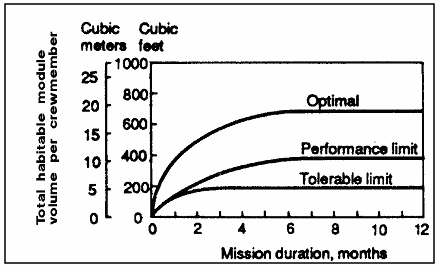
\includegraphics[scale=1.0]{./Figure/CrewModule/Crewvolume}
	\caption{Habitable volume per crew member as a function of mission duration \cite{Rudisill2008}}
	\label{fig:crewvolume}
\end{figure}
In the remainder of this report the crew habitable volume will be sized to the 'performance limit' indicated in figure \ref{fig:crewvolume}.